%Use one of the two documentclass lines depending on aspect ratio needed
% for 4x3 aspect ratio slides
%\documentclass{beamer}
%for 16x9 (modern wide screen) aspect ratio slides
\documentclass[aspectratio=169]{beamer}

% Oxford Maths theming
\usetheme{oxfordmaths}
\usepackage{tikz}
\usetikzlibrary{decorations.pathreplacing}
\usetikzlibrary{positioning, arrows.meta}
% \definecolor{oxfordblue}{RGB}{0,33,71}
% colours
\definecolor{softblue}{RGB}{232,238,246}
\definecolor{softpink}{RGB}{252,232,242}
\definecolor{softyellow}{RGB}{255,248,220}
\definecolor{softpurple}{RGB}{242,232,245}
\definecolor{softgreen}{RGB}{232,245,236}
\definecolor{softorange}{RGB}{255,239,222}
\definecolor{darkblue}{RGB}{0,33,71}
\definecolor{darkpink}{RGB}{155,65,105}
\definecolor{darkyellow}{RGB}{150,110,20}
\definecolor{darkpurple}{RGB}{95,55,120}
\definecolor{darkgreen}{RGB}{40,120,75}
\definecolor{darkorange}{RGB}{180,95,20}

% Set author etc info
\title[Efficient Spectral Computations] %short version of title for slide footer
{Efficient Algorithms for Infinite-Dimensional Spectral Computations} %full title for titlepage
\author{Maggie McCarthy \\ Supervisor: Prof. Patrick Farrell}
\institute{Mathematical Institute\\University of Oxford}
\date[5 June 2026]  %short date for slide footer
% {Really Great Conference, May 2024} %main date for title page,
                        %can overload it to show say 'Conference X, Date Y'


%% Now for the actual slides %%
\begin{document}

\begin{frame}[plain]
  \titlepage
\end{frame}

\begin{frame}{The Spectra of Linear Operators}
  % \framesubtitle{A bit more information about this}

  Consider a linear operator $A$ on a Hilbert space $H.$ The spectrum of $A$ is 
  \vspace{1em}
  $$ \text{Sp}(A) = \{ z \in \mathbb{C} \mid (A-zI)^{-1} \text{ does not exist as a bounded operator} \}.$$


\vspace{1em}

 Computing $\text{Sp}(A)$ is a fundamental problem in mathematics with many applications.

 \vspace{1em}


  \begin{figure}
      \centering
      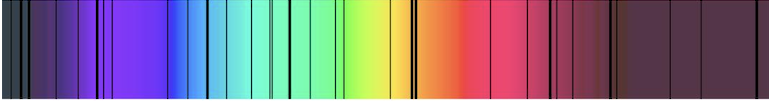
\includegraphics[width=1\linewidth]{spec_lines.png}
      \caption{\footnotesize The black `Fraunhofer lines' in a spectroscopic image of the sun's light correspond to the differences of eigenvalues of the Schrödinger operator for atoms such as H, Fe, Ca, Na, and Mg.}
      \label{fig:placeholder}
  \end{figure}

% Spectroscopic measurements such as these led to the discovery of the expanding universe.  
  
  
\end{frame}

\begin{frame}{$\text{Sp}(A)$ in Finite and Infinite Dimensions}

In finite dimensions, $A$ is an $n \times n$ matrix and $\text{Sp}(A)$ is a set of at most $n$ isolated points, which are the eigenvalues of $A.$
% $$\text{Sp}(A) = \{\lambda\in\mathbb{C}: Au=\lambda u \text{ for some }u\neq 0\}.$$

% $\text{Sp}(A)$ is a set of $n$ isolated points, which are the eigenvalues of $A.$

\vspace{2em}

In infinite dimensions, $\text{Sp}(A)$ may contain more than the eigenvalues of $A.$ It can have both discrete and continuous parts, making it much harder to compute. 

\vspace{2em}

For example, the right shift operator defined in $\ell^2,$
$$ A(u_1, u_2, \dots) = (0, u_1, u_2, \dots),$$
has a spectrum equal to the closed unit disk, but it has no eigenvalues. 


% The standard approach in infinite dimensions is to discretise the problem, compute the spectra of the corresponding finite-dimensional operator, and hope that the set of computed eigenvalues approaches $\text{Sp}(A).$ 

% \vspace{1em}

% To use finite element methodology to approximate spectra, we construct the variational formulation of $Au = zu$ in some infinite-dimensional space $V,$ project it into a finite-dimensional space $V_h,$ and solve the discretized problem for an approximation of $\text{Sp}(A).$


\end{frame}

% \begin{frame}{Computing $\text{Sp}(A)$ in infinite dimensions}

% The standard approach in infinite dimensions is to discretise the problem, compute the spectra of the corresponding finite-dimensional operator, $A_h,$ and hope that the set of computed eigenvalues approaches $\text{Sp}(A).$ 
% \vspace{1em}
% $$
% A
% \;\xrightarrow{\text{discretize}}\;
% A_h
% \;\xrightarrow{\text{solve}}\;
% \operatorname{Sp}(A_h)
% \approx
% \operatorname{Sp}(A).
% $$
% \vspace{0.75em}

% To use the finite element methodology, we construct the variational formulation of $Au = zu$ in some infinite-dimensional space $V,$ project it into a finite-dimensional space $V_h,$ and solve the discretized problem for an approximation of $\text{Sp}(A).$

% \end{frame}

\begin{frame}{Computing \(\operatorname{Sp}(A)\) in Infinite Dimensions}

\begin{columns}[T,onlytextwidth]

\begin{column}{0.60\textwidth}

The standard approach in infinite dimensions is to discretise $A$ with an $n$-dimensional operator, $A_h,$ and hope that $\text{Sp}(A_h)$ approaches $\text{Sp}(A).$

% to discretise the problem, compute the spectra of the corresponding finite-dimensional operator, $A_h,$ and hope that the set of computed eigenvalues approaches $\text{Sp}(A).$ 
% the problem with a finite-dimensional operator, $A_h,$ solve for $\text{Sp}(A_h),$ and hope that  $\text{Sp}(A_h),$
% \begin{itemize}
%     \item to discretise the problem 
%     \item compute the spectra of the corresponding finite-dimensional operator, $A_h,$ and
%     \item hope that the set of computed eigenvalues approaches $\text{Sp}(A).$
% \end{itemize}

\vspace{0.2cm}

\[
A
\;\xrightarrow{\text{discretize}}\;
A_h
\;\xrightarrow{\text{solve}}\;
\operatorname{Sp}(A_h)
\stackrel{?}{\approx}\;
\operatorname{Sp}(A).
\]
% \[
% A
% \;\xrightarrow{\text{discretize}}\;
% A_h
% \;\xrightarrow{\text{solve}}\;
% \operatorname{Sp}(A_h)
% \rightarrow \;
% \operatorname{Sp}(A) \text{ as } n \rightarrow \infty?
% \]

\vspace{0.3cm}

To use the finite element method, we
\begin{itemize}
    \item formulate the variational eigenproblem in an infinite-dimensional space \(V\),
    \item restrict the problem to a finite-dimensional space $V_h,$ and
    \item solve the discrete eigenproblem for $\text{Sp}(A_h).$
\end{itemize}

\vspace{0.2cm}

% In a basis, this gives a generalized matrix eigenproblem
% \[
% KU = \lambda_h MU.
% \]
\end{column}

\begin{column}{0.36\textwidth}
% \textbf{Reference}

% \vspace{0.2cm}

% \small
% D. Boffi,\\
% \emph{Finite Element Approximation of Eigenvalue Problems},\\
% Acta Numerica, 2010.

% \vspace{0.4cm}

% optional book/article image
\begin{center}
    
\includegraphics[width=0.75\linewidth]{daniele-boffi.jpg}

    \vspace{0.15cm}

    {\scriptsize
    \begin{minipage}{0.9\linewidth}
    \centering
    Reference: D. Boffi, \emph{Finite Element Approximation of Eigenvalue Problems}, Acta Numerica, 2010.
    \end{minipage}
    }
\end{center}
\end{column}

\end{columns}

\end{frame}

% \begin{frame}{How do we compute \(\operatorname{Sp}(A)\)?}

% In finite dimensions, \(A\) is an \(n\times n\) matrix and
% \[
% \operatorname{Sp}(A)=\{\lambda\in\mathbb{C}: Au=\lambda u
% \text{ for some }u\neq 0\}.
% \]

% \vspace{0.3cm}

% In infinite dimensions, \(\operatorname{Sp}(A)\) may contain more than eigenvalues:
% \[
% \text{point spectrum} \quad + \quad \text{continuous spectrum}.
% \]

% \vspace{0.3cm}

% The standard numerical approach is:

% \[
% A
% \quad \longrightarrow \quad
% A_h
% \quad \longrightarrow \quad
% \operatorname{Sp}(A_h)
% \approx
% \operatorname{Sp}(A).
% \]

% \vspace{0.3cm}

% For finite elements, choose \(V_h\subset V\), project the variational eigenproblem onto \(V_h\), and solve the resulting finite-dimensional eigenvalue problem.

% \end{frame}


% \begin{frame}{Dangerous pitfalls}

% \textbf{Spectral pollution:} The discretised operator has eigenvalues that converge to $z \notin \text{Sp}(A).$

% \vspace{1em}

% \textbf{Spectral invisibility:} Discretising the operator causes us to miss parts of its spectrum,
% even as the size of the discretisation increases.

% \vspace{1em}

% \textbf{Failure to compute the essential spectrum:}  In infinite dimensions, $\text{Sp}(A)$ may contain continuous, or essential, components that are extremely difficult or impossible to compute in a finite-dimensional setting.

    
% \end{frame}

\begin{frame}{Dangerous Pitfalls}

    

\begin{columns}[T,onlytextwidth]

% ---------------- LEFT COLUMN ----------------
\begin{column}{0.48\textwidth}
\small

\textbf{Spectral pollution:}  
The discretised operator has eigenvalues that converge to $z \notin \text{Sp}(A).$

\vspace{2em}

\textbf{Spectral invisibility:}  
Discretising the operator causes us to miss parts of its spectrum,
even as the size of the discretisation increases.


\vspace{2em}

\textbf{Failure to compute essential spectra:}  
In infinite dimensions, $\text{Sp}(A)$ may contain continuous or essential components that are extremely difficult or impossible to compute in a finite-dimensional setting.

\end{column}

% ---------------- RIGHT COLUMN ----------------
% \begin{column}{0.55\textwidth}
% \centering
% \resizebox{\linewidth}{!}{%
% \begin{tikzpicture}[x=1cm,y=1cm, every node/.style={font=\small}]
\begin{column}{0.49\textwidth}
\centering
\resizebox{!}{0.72\textheight}{%
    \begin{tikzpicture}[x=1cm,y=1cm, every node/.style={font=\small}]

% ---------- common dimensions ----------
\def\W{10.8}
\def\H{3.1}

% =========================================================
% 1. Spectral Pollution
% =========================================================
\begin{scope}[shift={(0,0)}]
    \draw[thick] (0,0) rectangle (\W,\H);

    \node[font=\bfseries] at (\W/2,2.7) {Spectral Pollution};

    \node at (\W/2,2.15) {\(\operatorname{Sp}(A)\)};
    \draw[decorate,decoration={brace,amplitude=5pt}] (1.7,1.7) -- (9.1,1.7);

    % true spectrum
    \draw[line width=0.8pt] (1.9,1.45) -- (4.6,1.45);
    \draw[line width=0.8pt] (5.8,1.45) -- (8.9,1.45);

    % computed spectrum
    \draw[dotted, line width=1.2pt] (1.8,0.9) -- (8.95,0.9);

    % spurious point
    \draw[gray] (5.15,0.9) circle (0.23);
    \fill (5.15,0.9) circle (0.08);

    \draw[->] (6.2,1.15) -- (5.4,0.97);
    \node at (7.4,1.15) {spurious limit};

    \node at (\W/2,0.25) {\(\operatorname{Sp}(A_h)\)};
    \draw[decorate,decoration={brace,mirror,amplitude=5pt}] (1.7,0.75) -- (9.1,0.75);
\end{scope}

% =========================================================
% 2. Spectral Invisibility
% =========================================================
\begin{scope}[shift={(0,-3.7)}]
    \draw[thick] (0,0) rectangle (\W,\H);

    \node[font=\bfseries] at (\W/2,2.7) {Spectral Invisibility};

    \node at (\W/2,2.15) {\(\operatorname{Sp}(A)\)};
    \draw[decorate,decoration={brace,amplitude=5pt}] (1.8,1.6) -- (9,1.6);

    % true spectrum
    \draw[line width=0.8pt] (1.9,1.45) -- (4.35,1.45);
    \draw[line width=0.8pt] (6.25,1.45) -- (8.65,1.45);

    % computed spectrum only sees one part
    \draw[dotted, line width=1.2pt] (6.25,1) -- (8.65,1);

    \draw[->] (3.1,1.1) -- (3.1,1.40);
    \node at (3.25,0.9) {missed spectrum};

    \node at (7.68,0.25) {\(\operatorname{Sp}(A_h)\)};
    \draw[decorate,decoration={brace,mirror,amplitude=5pt}] (6,0.8) -- (9,0.8);
\end{scope}

% =========================================================
% 3. Continuous and Essential Spectra
% =========================================================
\begin{scope}[shift={(0,-7.4)}]
    \draw[thick] (0,0) rectangle (\W,\H);

    \node[font=\bfseries] at (\W/2,2.7) {Continuous and Essential Spectra};

    \node[align=left] at (1.9,1.65) {discrete\\spectra};
    \fill (3.35,1.78) circle (0.06);
    \fill (3.70,1.45) circle (0.06);
    \fill (3.60,1.98) circle (0.06);

    \draw[line width=0.9pt] (3.55,0.5)
        .. controls (4.2,0.95) and (6.9,1.00) ..
        (7.7,1.70)
        .. controls (7.85,1.95) and (7.75,2.10) ..
        (7.82,2.35);

    \node[align=left] at (8.8,1.15) {continuous\\or essential\\spectra};
\end{scope}

\end{tikzpicture}%
}
\end{column}
\end{columns}

\end{frame}

\begin{frame}{An Example of Spectral Pollution: The Maxwell Eigenproblem}
Let $V = H_0(\operatorname{rot};U)$ and $U = (0, \pi)^2.$

\vspace{1em}

The variational formulation of the Maxwell eigenproblem is to find $\omega\in\mathbb R\setminus\{0\}$ and nonzero $\mathbf E \in V$ such that
% Let $V = H_0(\operatorname{rot};U)$ and $U = (0, \pi)^2.$ 
% \newline
% \textbf{Variational formulation:} Find $\omega\in\mathbb R\setminus\{0\}$ and a nonzero $\mathbf E \in V \text{ such that }$
% $$ \text{Find } \omega\in\mathbb R\setminus\{0\} \text{ and a nonzero } \mathbf E \in V \text{ such that }
$$\int_{U} \operatorname{rot}\mathbf E \,\, \overline{\operatorname{rot}\mathbf v} \, dx = \omega^2 \int_{U} \mathbf E \cdot \overline{\mathbf v} \, dx \qquad
\forall \mathbf v\in V.
$$

\vspace{1em}

The squares of the eigenvalues, $\omega^2,$ correspond to the Neumann eigenvalues of the Laplacian in $U.$ Thus,
$$ \omega^2 = n^2 + m^2 \qquad \text{for } n, m \in \mathbb{N}_0, \qquad (m,n) \ne (0, 0).$$ 
\end{frame}


\begin{frame}{An Example of Spectral Pollution: The Maxwell Eigenproblem}
Using standard Lagrange continuous piecewise linear elements yields spectral pollution:
% Using standard continuous piecewise-linear Lagrange elements for this problem produces spectral pollution.
\vspace{0.5em}
\begin{center}
\begin{minipage}{0.32\textwidth}
    \centering
    {\footnotesize \(N=4\)}
    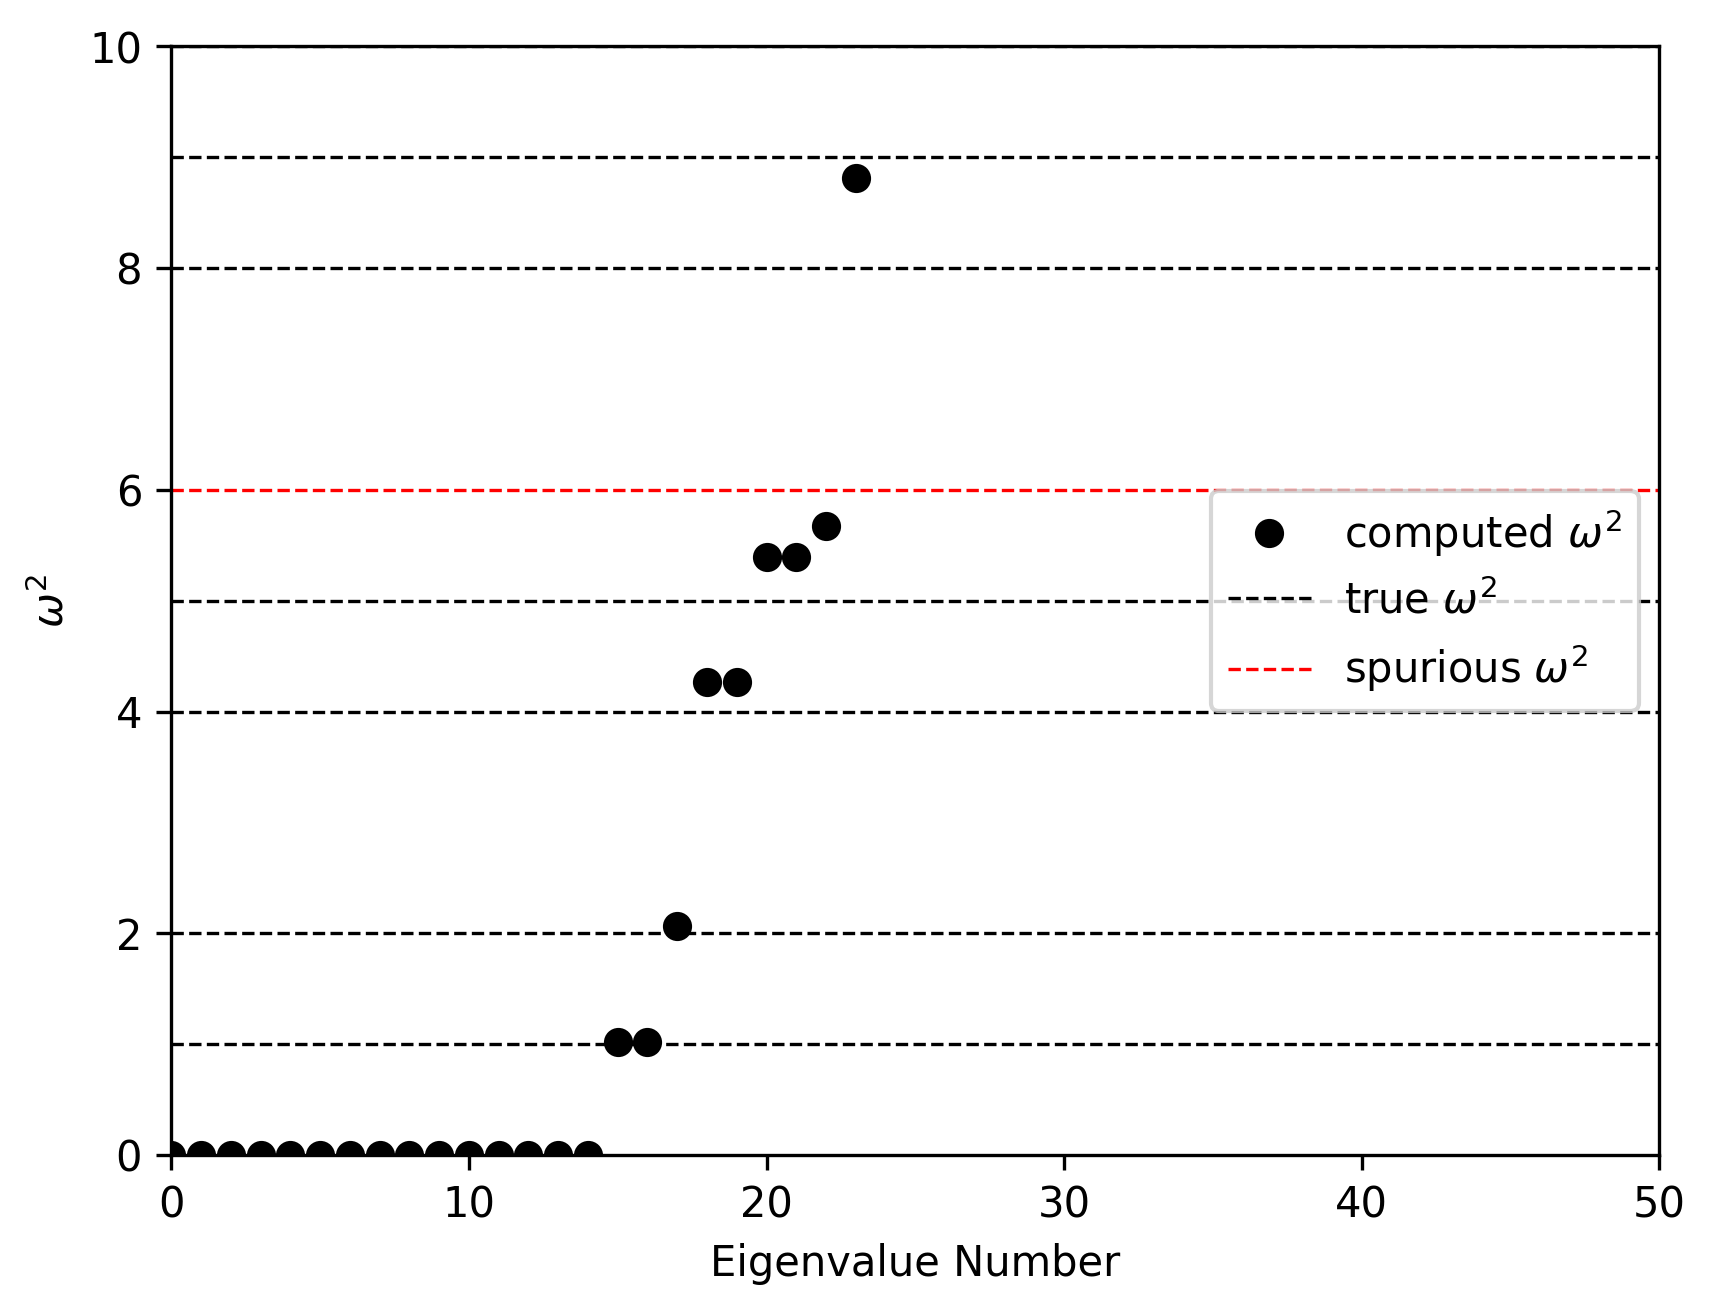
\includegraphics[width=\textwidth]{CrissCross_CG1_N4.png}
\end{minipage}
\begin{minipage}{0.32\textwidth}
    \centering
    {\footnotesize \(N=8\)}
    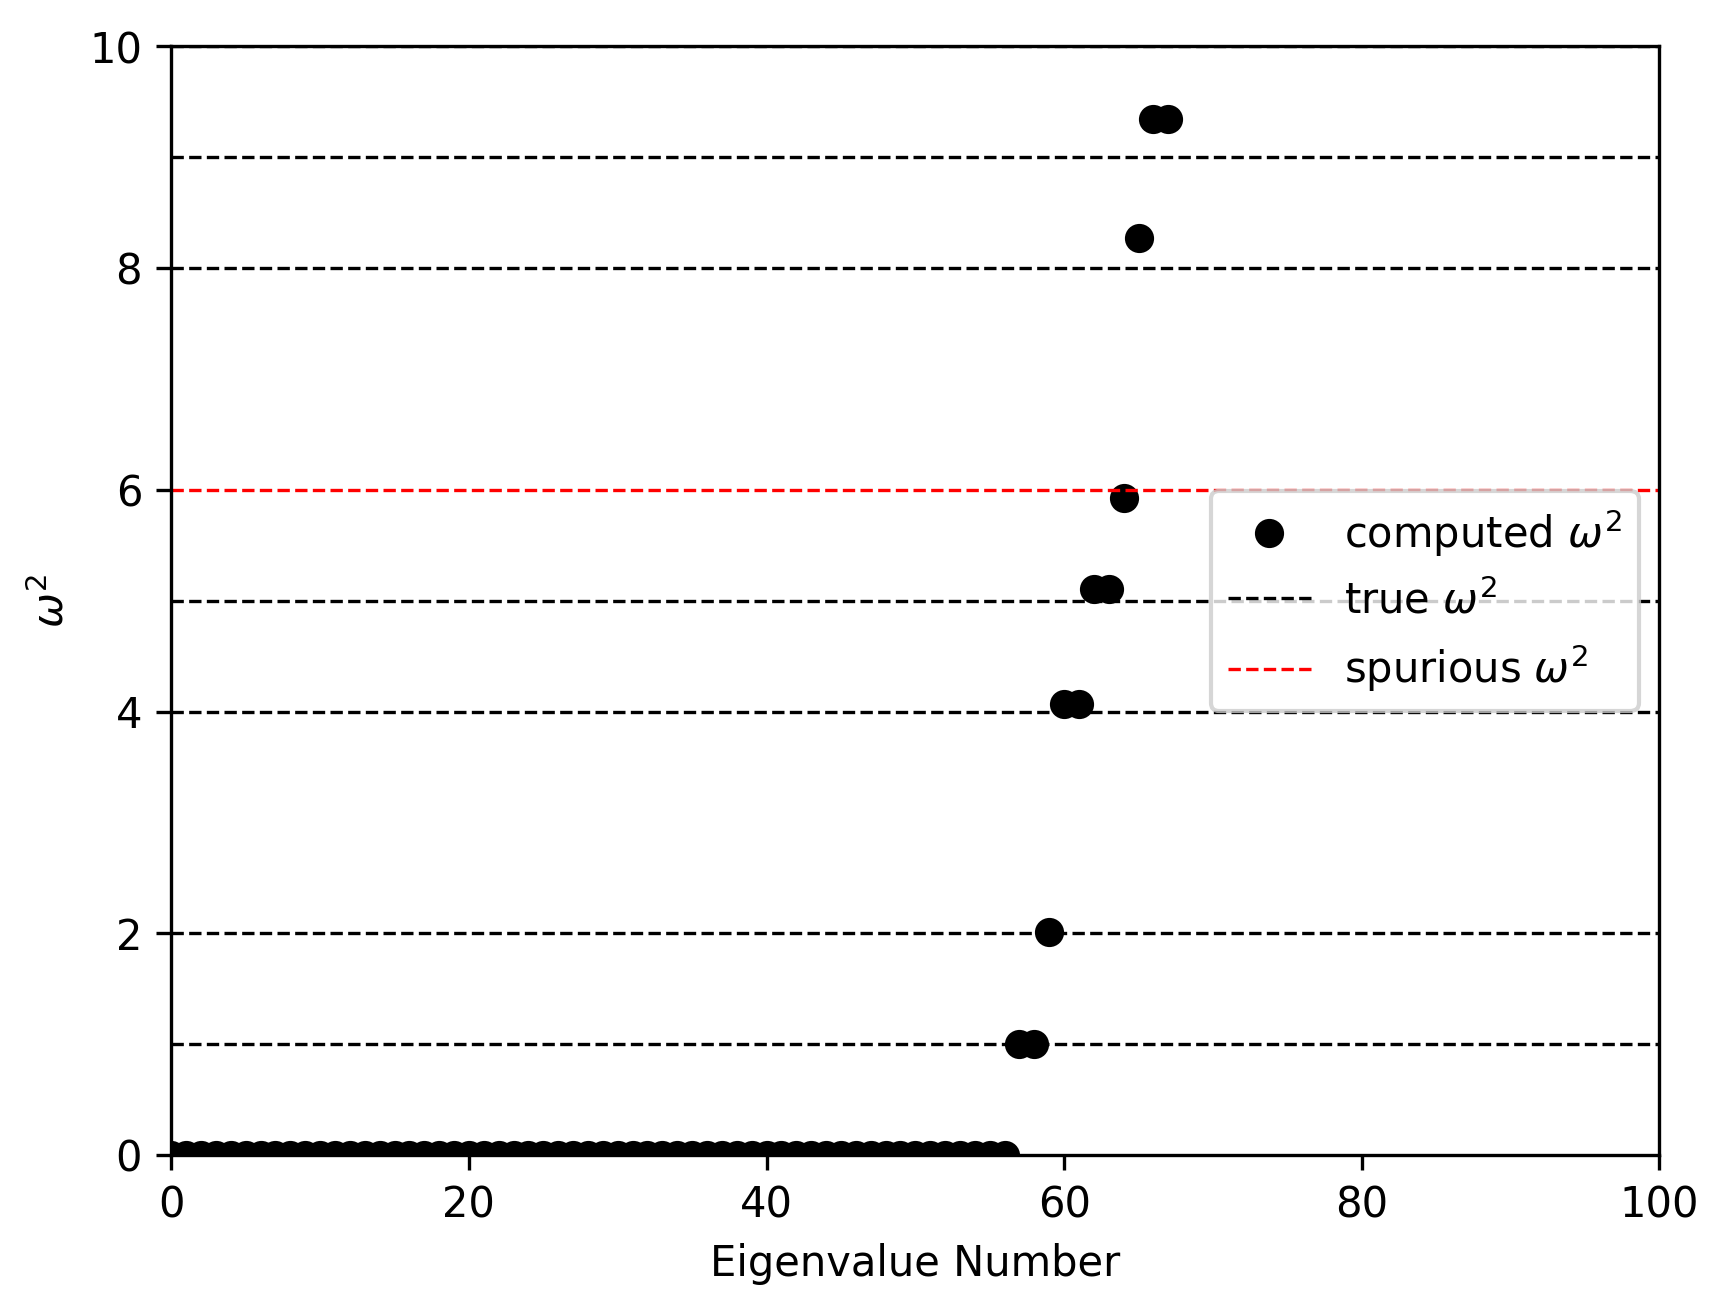
\includegraphics[width=\textwidth]{CrissCross_CG1_N8.png}

\end{minipage}
\begin{minipage}{0.32\textwidth}
    \centering
     {\footnotesize \(N=16\)}
    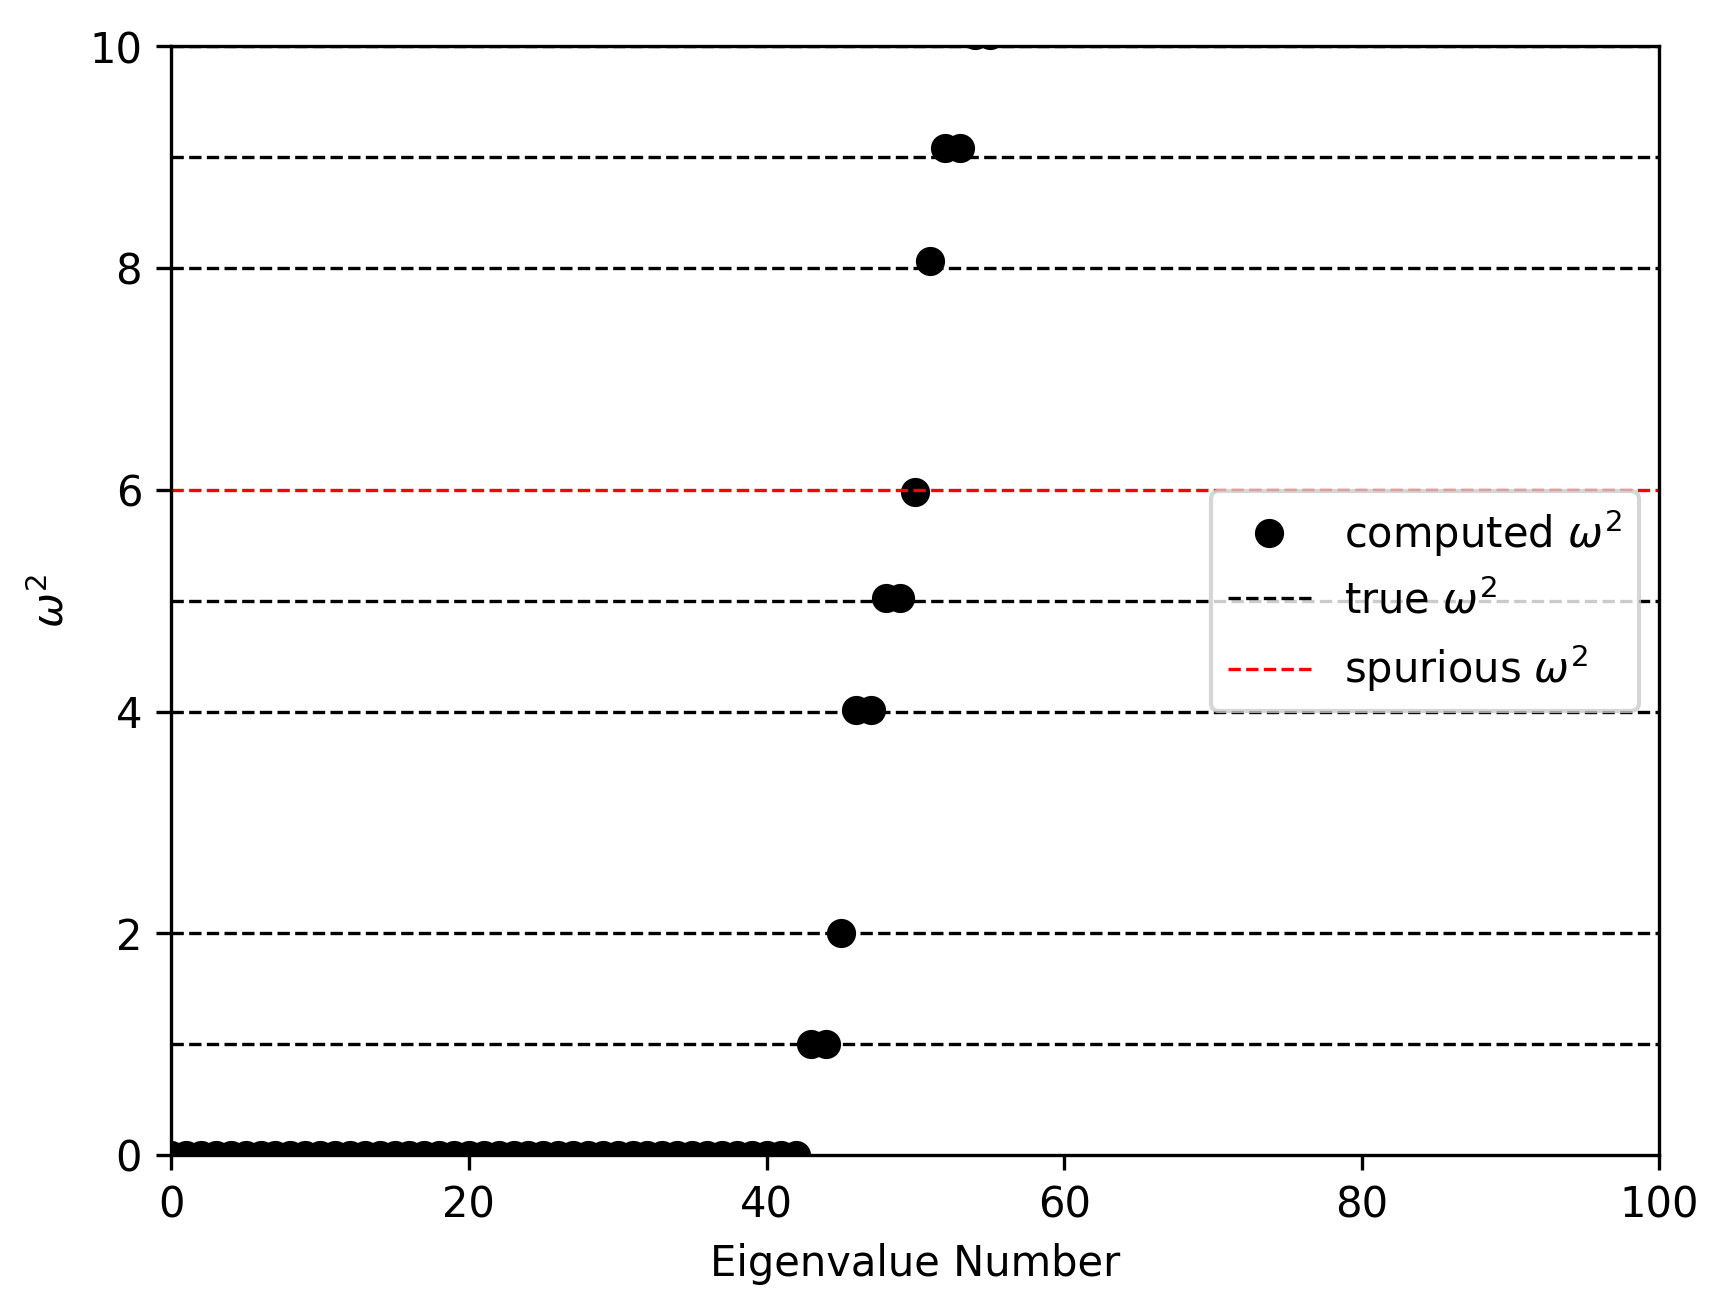
\includegraphics[width=\textwidth]{CrissCross_CG1_N16.png}
    
\end{minipage}
\end{center}
\vspace{0.5em}
In general, whether spectral pollution occurs depends on the choice of mesh and finite elements.
\end{frame}


% Let $U \subset \mathbb{R}^2.$ Find $\omega \in \mathbb{R}\setminus\{0\}$ and a nonzero $(\mathbf{E}, H) \in H_0(\text{rot} ; U) \times H(\mathbf{rot}; U)$ such that $$\mathbf{rot} \, \text{rot} \mathbf{E} = \omega^2 \, \mathbf{E} \qquad \text{ in } U \subset \mathbb{R}^2$$
% with
% $$ \mathbf{E} \cdot \mathbf{t} = 0,$$
% where 
% $$ E = (E_1, E_2)^T,$$
% $$ \mathbf{rot} E = \partial_x E_1 - \partial_y E_2, $$
% $$ \math$$


\begin{frame}{The Remedy}
    % A reliable algorithm for computing $\text{Sp}(A)$ should converge as the size of the discretisation, $n,$ tends towards infinity and guarantee that any point of the output is close to $\text{Sp}(A),$ up to an arbitrary small error tolerance. 
    % \end{itemize}
    % \begin{itemize}
    %     \item  converge as the size of the discretisation, $n,$ tends towards infinity.
    %     \item  guarantee that any point of the output is close to $\text{Sp}(A),$ up to an arbitrary small error tolerance. 
    % \end{itemize}

    \begin{columns}[T]

    \begin{column}{0.62\textwidth}
       % Matthew Colbrook at Cambridge has proposed an algorithm for infinite-dimensional spectral computation. In certain cases, his method converges to $\text{Sp}(A)$ and provides a local error bound, $E(n,z),$ on the distance to the spectrum, $ \text{dist}(z, \text{Sp}(A)) \le E(n, z).$  

    Matthew Colbrook at Cambridge has proposed an algorithm that, in certain cases, converges to $\text{Sp}(A)$ and provides a local error bound, $E(n,z),$ on the distance to the spectrum, $ \text{dist}(z, \text{Sp}(A)) \le E(n, z).$  
    % In certain cases, this algorithm can be proven to converge to the correct spectrum, so that neither spectral pollution nor spectral invisibility occur.

    \vspace{1em}

    The method is rooted in approximating
    $$  \gamma(z,A)=\min\left\{
\sigma_{\inf}(A-zI),
\sigma_{\inf}\left((A-zI)^*\right)
\right\},$$
where $\sigma_{\inf}(A) = 
\inf\left\{
\|Ax\| : x \in D(A),\ \|x\|=1
\right\}.$

 \vspace{1em}
This can be used to characterize $\text{Sp}(A)$ via
$$ \text{Sp}(A) = \{ z \in \mathbb{C} \mid \gamma(z, A) = 0 \}.$$

\end{column}
\begin{column}{0.38\textwidth}
% \centering
% \includegraphics[width=0.65\linewidth]{Image 2026-05-26 at 5.37 PM.png}

% \vspace{0.25em}
% {\tiny Reference: M. J. Colbrook. \emph{Infinite-Dimensional Spectral Computations: Foundations, Algorithms, and Modern Applications}. Cambridge University Press, 2026. Forthcoming}
% \end{column}
\begin{center}

    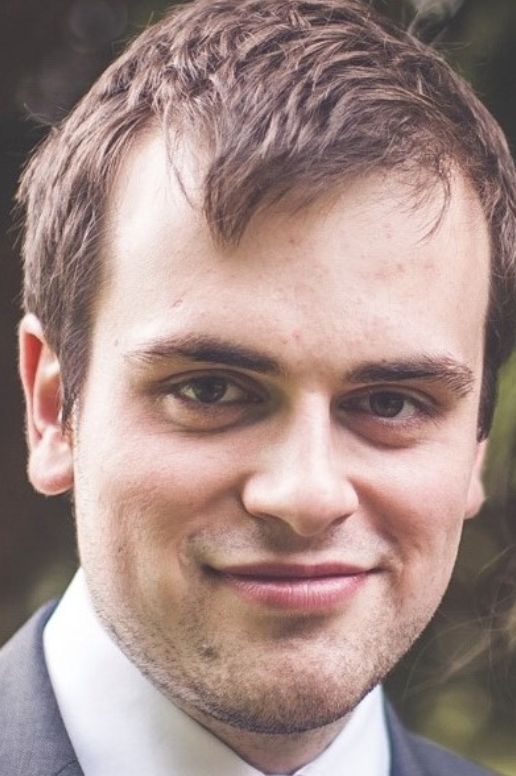
\includegraphics[width=0.5\linewidth]{matt.png}

    \vspace{0.15cm}

    {\scriptsize
    \begin{minipage}{0.9\linewidth}
    \centering
    Reference: M. J. Colbrook. \emph{Infinite-Dimensional Spectral Computations: Foundations, Algorithms, and Modern Applications}. Cambridge University Press, 2026. Forthcoming.
    \end{minipage}
    }
\end{center}
\end{column}

\end{columns}

\end{frame}

% \begin{frame}{The General Algorithm}

% % Using this characterization, the general idea of Colbrook's algorithm is as follows:
% % \vspace{0.5em}
% \begin{enumerate}
%     % \item Discretize the complex plane with a grid of $M$ points, denoted $\text{Grid}(M).$
%     \item Discretize the complex plane with a uniform grid covering a disc of radius $M,$ denoted $\text{Grid}(M).$
%     \vspace{1em}
%     \item For each $z \in \text{Grid}(M),$ compute an approximation of $\gamma(z, A),$ and the associated bound $ E(n, z).$ This often requires an approximation of the smallest eigenvalues of $(A-zI)^*(A-zI)$ and $(A-zI)(A-zI)^*.$
%     % For example, when $A$ is normal and has finite range, $E(n,z) \approx \lambda_{min}\left( (A-zI)^*(A-zI) \right).$
%     \vspace{1em}
%     \item When $z$ is sufficiently close to the spectrum, i.e., when $E(n, z)$ is sufficiently small, seek local minimizers of $E(n, \cdot)$ over the set of $w \in \text{Grid}(M)$ that are at a distance of at most $E(n, z)$ from $z.$
%     \vspace{1em}
%     \item The collection of local minimizers is the approximation of $\text{Sp}(A).$
% \end{enumerate}


\end{frame}



\begin{frame}{The General Algorithm}

\begin{center}
\begin{tikzpicture}[
    node distance=0.45cm,
    box/.style={
        draw,
        rounded corners,
        align=center,
        % text width=0.7\textwidth,
        minimum width=9.0cm,
        minimum height=0.85cm,
        font=\footnotesize,
        inner sep=5pt
    },
    sidebox/.style={
        draw,
        rounded corners,
        align=center,
        text width=0.20\textwidth,
        minimum height=0.85cm,
        font=\footnotesize,
        inner sep=5pt
    },
    arrow/.style={->, thick}
]


\node[box, draw=darkblue, fill=softblue]  (grid) {
Discretize the complex plane with a uniform grid \\ covering a disc of radius $M,$ denoted $\text{Grid}(M).$
};

\node[box, draw=darkpink, fill=softpink, below=of grid] (compute) { For each $z\in\text{Grid}(M),$ compute an approximation \\ of $\gamma(z, A),$ and the associated bound $ E(n, z).$
};

\node[sidebox, draw=darkyellow, fill=softyellow, right=0.5cm of compute] (eigvals) {
This often requires an approximation of the smallest eigenvalues of $(A-zI)^*(A-zI)$ and $(A-zI)(A-zI)^*.$}


\node[box, draw=darkgreen, fill = softgreen, below=of compute] (local) {
When $z$ is sufficiently close to the spectrum,  i.e., when $E(n, z)$ is \\ sufficiently small, seek local minimizers of $E(n, \cdot)$ over the set of \\ $w \in \text{Grid}(M)$ that are at a distance of at most $E(n, z)$ from $z.$
};

\node[box, draw=darkpurple, fill = softpurple,below=of local] (output) {
The collection of local minimizers is the approximation of $\operatorname{Sp}(A)$.
};

\draw[arrow] (grid) -- (compute);
\draw[arrow] (compute) -- (local);
\draw[arrow] (local) -- (output);

\draw[arrow] (compute.east) -- (eigvals.west);

\end{tikzpicture}
\end{center}

\end{frame}




\begin{frame}{Project Motivation}

\textbf{Motivating challenges:}
\begin{enumerate}
    \item To compute $E(n,z),$ we solve eigenproblems at each $z \in \text{Grid}(M).$ This is expensive.
    \vspace{0.5em}
    \item If the discretization of an eigenproblem is too coarse, $E(n,z)$ does not tightly bound $\text{dist}(z, \text{Sp}(A)).$ 
\end{enumerate}
% To compute $E(n,z),$ we solve eigenproblems at each $z \in Grid(N).$ If the discretization of the eigenproblem is too coarse, $E(n,z)$ does not tightly bound $\text{dist}(z, \text{Sp(A)}).$ 

\vspace{1em}

\textbf{Proposed approach:}
\begin{enumerate}
    \item To ease the computational effort of solving an eigenproblem at each $z \in \text{Grid}(M),$ we will explore and implement multilevel methods for eigenproblems.
    \vspace{0.5em}
    \item To compute a bound on $\text{dist}(z, \text{Sp}(A))$ to some desired accuracy, we will explore and implement an adaptive eigensolver. For example,  we plan to explore goal-based adaptivity based on the error of the smallest eigenvalue of each eigensolve.
\end{enumerate}
% % To overcome this issue, we aim to implement and adaptive eigensolver method that allows us to compute a bound on $\text{dist}(z, \text{Sp(A)})$ to some desired accuracy. For example, we plan to explore goal-based adaptivity based on the error on the smallest eigenvalue of each eigensolve.

% \vspace{2em}

% Furthermore, in an effort to ease the computational effort of solving sub-eigenproblems at each $z \in Grid(N),$ we will explore and implement multievel methods for eigenproblems.


\end{frame}


\begin{frame}{Project Aim: Efficient Spectral Computations}  
\begin{columns}[T]
\begin{column}{0.75\textwidth}
% The aims of this project are as follows:
% \vspace{1em}
\begin{enumerate}
    \item Perform a thorough \textbf{literature review} of the work done on computing the spectra of operators, on Colbrook's algorithm, on multilevel methods for eigenproblems, and on adaptive methods for eigenproblems. 
    \vspace{1em}
    \item \textbf{Implement Colbrook's algorithm}, ideally in Firedrake. 
    \vspace{1em}
    \item \textbf{Implement an adaptive multilevel method }for the eigensolve at each $z \in \text{Grid}(M).$ This solver will efficiently compute a bound on $\text{dist}(z, \text{Sp}(A))$ to within a guaranteed error tolerance.
\end{enumerate}
\end{column}
\begin{column}{0.25\textwidth}
% \centering
% \includegraphics[width=0.65\linewidth]{Image 2026-05-26 at 5.37 PM.png}

% \vspace{0.25em}
% {\tiny Reference: M. J. Colbrook. \emph{Infinite-Dimensional Spectral Computations: Foundations, Algorithms, and Modern Applications}. Cambridge University Press, 2026. Forthcoming}
% \end{column}
\begin{center}

    
\includegraphics[width=0.9\linewidth]{dragon.png}

    \vspace{0.15cm}

    {\scriptsize
    \begin{minipage}{0.9\linewidth}
    \centering
    The logo for Firedrake, an automated system for the solution of partial differential equations using the finite element method.
    \end{minipage}
    }
\end{center}
\end{column}
\end{columns}
\end{frame}



\begin{frame}{Short and Long Term Goals}

\textbf{Recent work:}
\begin{itemize}
    \item Learning about the spectra and pseudospectra of linear operators.
    \item Learning about the discretisation and computation of the spectra of operators using the finite element method. 
\end{itemize}

% \textbf{Next steps:}
% \begin{itemize}
%     \item A literature review of multilevel methods for eigenproblems.
%      \item A literature review of Colbrook's algorithm.
%      \item Implementation of Colbrook's algorithm in Firedrake.
%      \item A literature review of adaptive eigensolves.
%      \item Implementation of an adapted multilevel method for the eigensolves in Colbrook's algorithm.
% \end{itemize}
% \end{frame}

% \textbf{Recent work:}
% \begin{itemize}
%     \item Learning about the spectra and pseudospectra of linear operators.
%     \item Learning about the discreization and computation of the spectra of operators using the finite element method. 
% \end{itemize}

\textbf{The next step:}
\begin{itemize}
    \item A literature review of multilevel methods for eigenproblems.
\end{itemize}
\textbf{Long term goals:}
\begin{itemize}
     \item A literature review of Colbrook's algorithm.
     \item Implementation of Colbrook's algorithm in Firedrake.
     \item A literature review of adaptive eigensolves.
     \item Implementation of an adapted multilevel method for the eigensolves in Colbrook's algorithm.
\end{itemize}
\end{frame}

\begin{frame}{Extra: The Spectra of the Shift Operators}
    Consider the $\ell^2$ sequence space. This is a Hilbert space with norm $\| x \|^2 = \sum_{n=1}^{\infty} |x_n|^2$ and inner product $\langle x, y \rangle = \sum_{n=1}^{\infty} x_n \overline{y_n}.$

    \vspace{1em}

    Define the left and right shift operators on $\ell^2$ as 
    $$ L(x_1, x_2, \dots) = (x_2, x_3, \dots) \,\, \text{ and } \,\, R(x_1, x_2, \dots) = (0, x_1, x_2, \dots),$$
    respectively.

    \vspace{1em}
     
    Notice that $L^* = R$ and $\| R \| = \|L\| = 1.$

    \vspace{1em}

        When $A$ is bounded,
     $\text{Sp}(A) \subset \{ z \in \mathbb{C} \mid |z| \le \|A\| \}.$
    Thus,
     $$ \text{Sp}(L),  \text{Sp}(R) \subset \{ z \in \mathbb{C} \mid |z| \le 1 \}.$$
    
\end{frame}

% \begin{frame}{Continued: The Spectra of the Shift Operators}

%     When $A$ is bounded,
%     $$ \text{Sp}(A) \subset \{ z \in \mathbb{C} \mid |z| \le \|A\| \}.$$

%     Since $\|L \| = \|R\| = 1,$
%     $$ \text{Sp}(L) \subset \{ z \in \mathbb{C} \mid |z| \le 1 \}$$
%     and 
%     $$ \text{Sp}(R) \subset \{ z \in \mathbb{C} \mid |z| \le 1 \}.$$

% \end{frame}

\begin{frame}{Continued: The Spectra of the Shift Operators}

    The eigenvalues of $L$ are found by solving $Lx = \lambda x$ for any $\lambda \in \mathbb{C}$ and a nonzero $x \in \ell^2.$

     \vspace{0.5em}

    Thus, the eigenvectors are of the form
    $$ x = x_1 (1, \lambda, \lambda^2, \dots)$$
    and must satisfy
    $$ |x_1|^2 \sum_{n=0}^{\infty} |\lambda|^{2n} < \infty.$$


 From this we find that
    $$\Gamma(L) = \text{set of eigenvalues of } L = \{ \lambda \in \mathbb{C} \mid |\lambda| < 1 \} \subset \text{Sp}(L).$$

     \vspace{0.5em}

    Since the spectrum of a bounded operator is closed, the closed disk must also be in $\text{Sp}(L).$ Thus,  $ \text{Sp}(L) \supset \{ z \in \mathbb{C} \mid |z| \le 1 \},$  $ \text{Sp}(L) \subset \{ z \in \mathbb{C} \mid |z| \le 1 \},$ and so
     $$ \text{Sp}(L) = \{ z \in \mathbb{C} \mid |z| \le 1 \}.$$

\end{frame}

\begin{frame}{Continued: The Spectra of the Shift Operators}

    The eigenvalues of $R$ are found by solving $Rx = \lambda x$ for any $\lambda \in \mathbb{C}$ and a nonzero $x \in \ell^2.$
     \vspace{1em}
     
    In doing so we find that the eigenvectors must satisfy
    $$ (0, x_1, x_2, \dots) = \lambda(x_1, x_2, \dots).$$ 
    % Equivalently,
    % $$ \lambda x_1 = 0, \,\, \lambda x_2 = x_1, \,\, .\dots$$
   The only solution is $x=0$ which cannot be an eigenvector. Thus, $R$ has no eigenvalues.

     \vspace{1em}

    When $A$ is closed and densely defined, $\text{Sp}(A^*) = \{\overline{z} \mid z \in \text{Sp}(A) \}.$ Here, $L$ and $R$ are bounded operators on all of $\ell^2$ and $L^* = R$. Thus, 
    $$ \text{Sp}(R) = \{\overline{z} \mid z \in \text{Sp}(L) \} = \{ z \in \mathbb{C} \mid |z| \le 1 \}.$$



\end{frame}



\end{document}
